\chapter{Introduction}
\label{cha:introduction}

A network is a set of objects structured such that some pairs of the objects are related in some sense. Networks provide a ubiquitous way to organize a diverse set of real-world information from social relationships to generating stations in a power grid. 

A financial network concept originated for describing and modelling complex systems of financial relationships between financial institutions to resist financial turmoil and maintain financial stability efficiently.  The concept has proven to be valid on a broad set of tasks such as contagion and system risk, the formation of interbank markets and characterization of current financial systems since it allows to keep track and foresee adverse spillover effects within the network.

Complex financial networks can describe a variety of real-world scenarios. For example, in retail banking network's participants are consumers and enterprises of different size and purpose, who establish relationships by transferring assets to each other. Participants of the interbank networks are individuals and legal entities. The current thesis considers a financial transaction network where nodes are anonymous users/accounts/companies and edges are committed transactions. 

A node segmentation is of the main challenges in network analysis. The traditional node segmentation approach is usually based on explicitly determined network's attributes.
However, either such segmentation might provide limited explanations, or there might be no available attributes of a network. One prominent example of recent years is a cryptocurrency financial transaction network, where participants are represented by accounts, and their personal information is securely encrypted. The traditional analysis approach for node segmentation here would be to calculate common graph metrics such as in-degree, out-degree, clustering coefficient, etc. and use them as attributes. Unfortunately, these traditional metrics do not consider the local neighbourhood structures of the nodes in a network and therefore neglect valuable information. 

This thesis presents a concept for node segmentation in financial transaction networks. The concept leverages network local structural information, time attribute, and one of the common graph metric - degree. The concept is implemented in the form of a data science pipeline and utilizes the state-of-the-art unsupervised machine learning techniques. The pipeline combines neural networks and the advantages of financial network concept for financial data analysis. The outcome of the pipeline are segments of nodes (users) grouped according to the combination of user-selected features:
\begin{enumerate}
  \item network local structural information,
  \item edges-associated time attribute,
  \item nodes-associated degree attribute. 
\end{enumerate}
Real-World financial transaction networks are typically dynamic networks where each edge (transaction) has a timestamp of emergence. It is considered as a time attribute characterizes a network evolution.

Such segmentation might become useful in some research areas as it provides an overview of financial network participants in terms of their local structures, times of activity, and global structural roles. For instance, it can serve for fraud detection to reveal such notorious fraud techniques as Ponzi schemes and Pyramid schemes which once have been flourishing until they have been disclosed and declared illegal. The fraudsters usually proceed according to the same scenario and were characterized by similar behaviour, which can be observed in the financial network structure and, thus, captured by the proposed method. Another potential application scenario might be appealing for financial authorities who can provide their customers with new business opportunities according to their mined network segment.

Overall, this work addresses the problem of segmentation participants in a dynamic financial transaction network. The ultimate value of this work is designing the method which finds segments of nodes grouped by a similar local neighbourhood structure, the global structural attribute - degree, and an overlapping time of activity.

\section{Motivation}
\label{Motivation}
The incentive to create a method for financial network studying was the utter privacy of the financial transaction data worldwide. Only rarely such data became public and, therefore, available for research. Sometimes financial transaction data become disclosed without personally identifiable information~\footnote{\textbf{Personally identifiable information} is any information relating to an identifiable person or can be used to de-anonymizing anonymous data~\cite{McCallister:2010:SGP:2206206}.} (some examples are mentioned in the~\ref{Financial Networks}). Generally, a financial transaction is a pair of users: a sender - a party who sent an asset and a receiver - a party who received this asset. Some parties can be senders and receivers in different transactions. It allows to model anonymized financial transaction data as a directed graph, where vertices are users and edges are transactions between pairs of users from a sender to a receiver (~\autoref{fig:Fig27}). 

\begin{figure}[!ht]
	\centering
	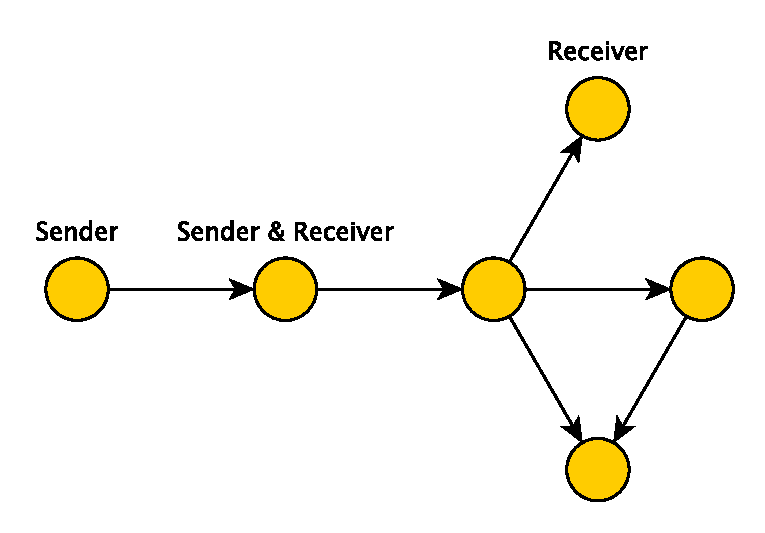
\includegraphics[width=0.48\textwidth]{images/Fig27.pdf}\\
	\caption{Directed graph built on transaction data}
	\label{fig:Fig27}
\end{figure}

Despite the lack of parties' characteristics in the original data, a graph representation is yet powerful, as it provides information about the interaction between parties and reveals the structure of established relationships in the form of a financial network. Having data represented as a graph, it can be exposed to all state-of-the-art network analysis approaches which exploit a network structure. Thus, the financial transaction data with limited information can be extensively studied based on its network structure.
Time is another crucial component of a real-world anonymized financial transaction data which is usually available for analysis. It transforms the underlying network from static to dynamic and allows to cluster users based on both structural and their activity time components.

The opportunity to represent sensitive financial data in a way enabling additional feature retrieval in order to study such data became the motivation for the creation of the current concept.

\section{Idea}
Considering the fact of the high sensibility of financial data and, therefore, its common limited accessibility, the idea of this thesis is splitting financial transaction network participants into segments according to their local structural similarity, global structural similarity and time of activity within the network. 
A number of financial network studies engage traditional Network Analysis approaches to obtain structure-based features including the computation degree, clustering coefficient, PageRank centrality etc. for each node~\cite{ContagionFinNets} ~\cite{StatisticAnalysisFinNetworks}. Although this manual feature engineering provides an insightful outcome in some cases, in others it may be not really helpful or computationally feasible. A method designed in this thesis determines similar participants of a network by their local neighbourhood structures, a global degree attribute, and time attribute. It forms respective segments of nodes making use of an automated feature engineering for networks with semi-supervised algorithms. The method consists of tree main stages: automated feature learning from a network, reducing the dimensionality of the learned continuous space, cluster analysis of nodes' representations in the low-dimension space. 

\subsection{Network feature engineering}
A traditional approach to obtain the structure-based features includes the computation of each network participants' in-degree, out-degree, clustering coefficient, etc. Clustering the nodes based on such features can help in determining segments of similar nodes, but it does not consider the local neighbourhoods of the nodes, which can play an essential role for user segmentation in financial networks and reveal hidden similarities among the participants. Another drawback of the traditional approach is a computation expense. A modern fast alternative to a network feature engineering is network embedding - general method, that aims at learning a low-dimensional latent representation of nodes in a network. Specifically, each node is assigned a dense vector representation based on its local neighbourhood in the feature space and encode community structure as had been shown in ~\cite{chen2018tutorial}. The major advantages over traditional network feature extraction approach are the ability to process large-scale networks in a shorter time, community aware feature learning, producing continuous feature representation space with a number of standard distance metrics and thereby allowing smooth decision boundaries between communities. The network embedding approach is the core of automated feature learning in this master thesis.

Real-world financial networks are constantly evolving, therefore, it is crucial to consider a time component in the network feature learning. However, the majority of the network embedding methods process only static networks, while real-world problems require to preserve both structural information about nodes' neighbourhoods and its operating dynamics. A Node2vec framework developed by Grover and Leskovec ~\cite{node2vec} pioneered alongside some others in the efficient automated feature learning. The analytical usefulness of Node2vec is in building vector representation for a node exploiting the unique flexible neighbourhood sampling strategy, the benefits of which will be discussed in details in \ref{Node2vec}. Originally the framework is intended for static networks. This fact limits its practical application. This master thesis presents a new modification of Node2vec framework which can process a dynamic network and learn features benefiting from its sampling strategy and a time component.

\subsection{Dimensionality reduction}
Dimensionality reduction is the transformation of high-dimensional data into a meaningful representation of reduced dimensionality. Such techniques gained popularity because they help to mitigate undesired properties of high-dimensional space.

The reference linear methods of dimensionality reduction such as PCA or LDA remain ubiquitously used since the last century because of their simplicity and clear interpretability. However, a number of nonlinear dimensionality reduction techniques have been proposed recently in order to better handle real-world data (e.g. t-distributed stochastic neighbor embedding ~\cite{maaten2008visualizing}, uniform manifold approximation and projection ~\cite{mcinnes2018umap}). A concept developed in the current thesis exploits three different linear and nonlinear dimensionality reduction techniques interchangeably. They are described in \ref{Dimensionality Reduction} and used to produce a low-dimensional representation of high-dimensional feature space.

\subsection{Cluster analysis}
The purpose of a cluster analysis is to divide input data into meaningful groups (clusters) so that the objects within a group are similar or related to one another and different from or unrelated to the objects in other groups. Resulting clusters capture the "natural" structure of the data. Clustering is very sensitive to the dimensionality of a processed space. In 1961 Richard Bellman in his book ~\cite{bellman2015adaptive} first identified the term 'curse of dimensionality' referring to the impossibility of optimizing a function of many variables by a brute force search on a discrete multidimensional grid (the number of grid points increases exponentially with dimensionality). Therefore, clustering is applied after the dimensionality reduction step in the frame of the concept in this work. Two clustering techniques - density-based and partitional clustering - are performed interchangeably at the final stage of the concept and described in~\ref{Cluster Analysis}.

\section{Aim and objective}
There is a variety of supervised machine learning methods for Network Analysis based on a set of explicitly given features and/or set of labels. As mentioned above, it is not always possible to have such data or to rely on its authenticity dealing with financial networks. Over recent years, the unsupervised machine learning methods demonstrated their efficiency upon a condition of deficiency of input information. 
One of the bases for feature extraction in unsupervised learning is an item context. For instance, in the case of Semantic Analysis, item context allows to distinguish between the same words having different semantic meaning (Word2vec~\cite{SKIP-GRAM-MODEL}). In case of Network Analysis, a structure of a nearest neighbourhood of a node provides contextual information. 
Though real-world cases in the financial domain are not based on data described by exhaustive feature set, network embedding approach opens up various ways to derive sense out of the raw data that can be represented as a network. Thereby, having no explicit features or data labels, it is still possible to apply network embedding unsupervised learning and derive clusters of nodes which are similar in terms of their neighbourhood structure. It may be highly relevant for the purposes below.
\begin{enumerate}
\item User segmentation based on local neighbourhoods structural similarities and other available graph attributes.
\item Fraud detection based on groups of participant, which are interacted within the similar local neighbourhoods, during the same time period and with roughly the same number of users. Ones one from a group was implicated in fraud, it is worth to pay close attention to other group's participants.
 \end{enumerate}
Unsupervised methods are on high demand for exploring financial transaction data sets since they require minimal number of features such as transfers between a sender and receiver and timestamps of these transfers. This information is usually available the real-world cases.

Various researchers have contributed to the subject by exploring the inherent structure of networks. Lei Tang and Huan Liu in ~\cite{tang2011leveraging} developed a framework for studying heterogeneous social media network based on the network structure. Huang et al in ~\cite{DeepEmbeddingNetworkforClustering} attempted to mine network representations most suitable for cluster analysis and evaluated their approach against the most common cluster techniques and benchmarking data sets. In fact, it is difficult to choose the best network embedding and clustering techniques for segmentation of network participants. Therefore, the developed concept provides a choice among several techniques at each data processing stage. The final results from every possible sequence of techniques are compared to each other. The result with the best score points to the best choice of techniques and their hyperparameters. Only the first stage for the network embeddings learning do not provide a choice of techniques, instead, it allows to choose the relevant graph attributes for learning. 

The majority of existing network embedding methods such as Node2vec~\cite{node2vec}, LINE~\cite{tang2015line}, DeepWalk~\cite{perozzi2014deepwalk} generally exploit a random walk model to learn each node's local neighbourhood. As network nodes are uniquely identified within a network, methods fulfil a homophily hypothesis~\cite{fortunato2010community}: placing embeddings for nodes that are highly interconnected and belong to similar network communities close to each other. An important attribute of real-world networks is time, which describes a network evolution and can contribute a lot to a feature learning. Some dynamic network embedding methods have been recently proposed, e.g. DynamicTriad~\cite{zhou2018dynamic} learns embedding via triadic closure process. The method processes a network by snapshots in every time period and may be slow on large networks.

The overall goal of the work is to present a concept for a users segmentation which reveals new similarities among nodes (users) of a network based on combination of their local neighbourhood structures, time and/or global structural attribute. The contributions of the thesis are:
\begin{itemize}
\item An overview of the state-of-the-art methods for network embedding learning, dimesionality reduction, and clustering.
\item A novel sampling strategy for network embedding, which incorporates local neighbourhoods' structures, time attribute, and global structural attribute (degree) .
\item Implementation of the proposed concept in the form of a multi-staged data science pipeline, which can process any network.
\item The performance evaluation strategy designed for the implemented pipeline
\item Interpretation of the final results produced by the pipeline on a real-world financial data set.
 \end{itemize}
 
\section{Application scenario}
The central concept as well as its implementation in general  can be applied to any kind of networks consisted of nodes connected by edges. The approach itself is domain-independent and does not require any specific adjustment to a subject area. The difference comes in the result interpretation as the revelling patterns are based on user-specific information within a given network.

From mathematical prospective, the concept is able to consume undirected/directed, unweighted/weighted dynamic/static multigraphs with loops. However, in the current work, it will be tested and evaluated on the undirected, unweighted dense multigraph.

A crucial limitation of the concept relates to network density. As the sampling strategy of the feature engineering method uses a random walk on local neighbourhoods of nodes in a network, it implies to process network which nodes are sufficiently connected by edges. In case of a network consists of many disconnected one-node components, a random walk is not able to traverse their local neighbourhoods through adjacent edges and derive representative samples to generate vector representations for such nodes. 

The developed method serves for analysis of real-world networks which are usually characterized by a short average shortest path and a high clustering coefficient comparing to a random network. A network feature learning will not extract any valuable features in case of the initial network structure is uniform across the network. Therefore, the concept is evaluated on a real-world dynamic network.

\section{Summary}
This chapter introduced the thesis, outlined the main idea behind the current work and set up the main motivations and objectives.

The following chapter presents a brief overview of the state-of-the-art approaches used in the present concept. It provides insights into recent literature describing current scientific achievements in the network embedding, dimensionality reduction, and cluster analysis. After that, a reader will find the description of the central concept along with its prototypical implementation details. The rest of the thesis is devoted to results evaluation, interpretation following by a brief summary in conclusion.